\section{The homological perturbation lemma in the BV formalism}\label{BV.HPL}

There is a natural toolkit from homological algebra that makes the manipulations in section \ref{BV.Wick} appear more systematic and less {\it ad hoc}. In particular, we want a technique to solve the basic problem:
\begin{quote}
If we know the cohomology $H^*(V,d)$ of some complex $(V,d)$, is there a method for computing the cohomology $H^*(V, d + \delta)$ where $\delta$ is some ``small" perturbation of the original differential?
\end{quote}
This problem appears frequently in mathematics; the spectral sequence of a double complex can be viewed as a tool for relating the horizontal cohomology to its ``perturbation," the full double complex. For us, we have the classical BV complex and its deformation, the quantum BV complex.

\subsection{Reminder on homological perturbation theory}

The homological perturbation lemma provides an answer to the problem but requires some extra control over the original complex.

\begin{definition}
A {\em contraction} (or {\em strong deformation retract}) consists of the following data:
\begin{enumerate}
\item[(i)] a pair of complexes $(V, d_V)$ and $(W, d_W)$;
\item[(ii)] a pair of cochain maps $\pi: V \to W$ and $\iota: W \to V$;
\item[(iii)] a degree $-1$ map of graded vector spaces $\eta: V \to V$.
\end{enumerate}
This data must satisfy:
\begin{enumerate}
\item[(a)] $W$ is a retract of $V$, so $\pi \circ \iota = \One_{W}$;
\item[(b)] $\eta$ is a chain homotopy between $\One_V$ and $\iota \circ \pi$, so
\[
\iota \circ \pi - \One_V = d_V \eta +\eta d_V = [d_V,\eta];
\]
\item[(c)] the {\em side conditions}
\[ 
\eta^2 = 0, \; \eta \circ \iota = 0, \text{ and } \pi \circ \eta = 0.
\]
\end{enumerate}
We draw this data as
\begin{equation*}\label{contraction}\tag{$\ast$}
  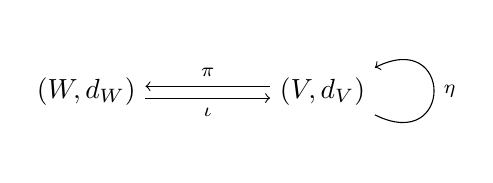
\begin{tikzpicture}[baseline=(L.base),anchor=base,->,auto,swap]
     \path node (L) {$(W,d_W)$} ++(3,0) node (M) {$(V,d_V)$} 
     (M.mid) +(0,.075) coordinate (raise) +(0,-.075) coordinate (lower);
     \draw (L.east |- lower) to node {$\scriptstyle \iota$} (M.west |- lower);
     \draw (M.west |- raise) to node {$\scriptstyle \pi$} (L.east |- raise);
     \draw (M.south east) ..controls +(1,-.5) and +(1,.5) .. node {$\scriptstyle \eta$} (M.north east);
  \end{tikzpicture}\end{equation*}
and use it as a visual shorthand throughout the text.
\end{definition}

\begin{definition}
A {\em perturbation} of a complex $(V,d_V)$ is a degree 1 map $\delta: V \to V$ such that $(d_V + \delta)^2 = 0$. A {\em small perturbation of a contraction} (using the notation in (\ref{contraction})) is a perturbation of $V$ such that $\One_V - \delta \eta$ is invertible or, equivalently, if $\One_V - \eta \delta$ is invertible.
\end{definition}

With these definitions in hand, we now introduce the useful trick.

\begin{theorem}[Homotopy Perturbation Lemma]
Given a small perturbation $\delta$ of a contraction, there is a new contraction 
\begin{equation*}
  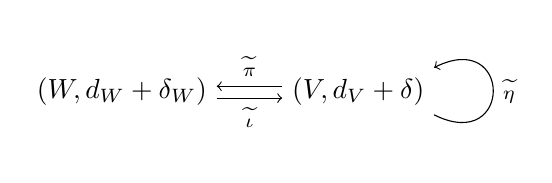
\begin{tikzpicture}[baseline=(L.base),anchor=base,->,auto,swap]
     \path node (L) {$(W,d_W + \delta_W)$} ++(3,0) node (M) {$(V,d_V + \delta)$} 
     (M.mid) +(0,.075) coordinate (raise) +(0,-.075) coordinate (lower);
     \draw (L.east |- lower) to node {$\scriptstyle \widetilde{\iota}$} (M.west |- lower);
     \draw (M.west |- raise) to node {$\scriptstyle \widetilde{\pi}$} (L.east |- raise);
     \draw (M.south east) ..controls +(1,-.5) and +(1,.5) .. node {$\scriptstyle \widetilde{\eta}$} (M.north east);
  \end{tikzpicture}
\end{equation*}
where
\begin{eqnarray*}
\delta_W &=& \pi \circ (\One_V - \delta \eta)^{-1} \circ \delta \circ \iota, \\
\widetilde{\iota} & = & \iota + \eta \circ (\One_V - \delta \eta)^{-1} \circ \delta \circ \iota, \\
\widetilde{\pi} & = & \pi + \pi \circ (\One_V - \delta \eta)^{-1} \circ \delta \circ \eta, \\
\widetilde{\eta} & = & \eta + \eta \circ (\One_V - \delta \eta)^{-1} \circ \delta \circ \eta.
\end{eqnarray*}
In short, there is a perturbed contraction.
\end{theorem}

We recommend \cite{Crainic} as a succinct reference for this lemma and some generalizations. In particular, one can work with general homotopy equivalences rather than contractions, but we do not need that level of generality.

\subsection{Applying perturbation theory in the BV formalism}

In the general situation of the BV formalism, we have two complexes, the classical observables 
\[
\obscl = (V,d)
\] 
and the quantum observables 
\[
\obsq = (V[[\hbar]], d_q  := d + \hbar d_1 + \hbar^2 d_2 + \cdots).
\] 
If we have a contraction of the classical observables, e.g.,
\[
  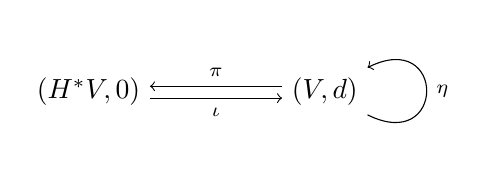
\begin{tikzpicture}[baseline=(L.base),anchor=base,->,auto,swap]
     \path node (L) {$(H^* V,0)$} ++(3,0) node (M) {$(V,d)$} 
     (M.mid) +(0,.075) coordinate (raise) +(0,-.075) coordinate (lower);
     \draw (L.east |- lower) to node {$\scriptstyle \iota$} (M.west |- lower);
     \draw (M.west |- raise) to node {$\scriptstyle \pi$} (L.east |- raise);
     \draw (M.south east) ..controls +(1,-.5) and +(1,.5) .. node {$\scriptstyle \eta$} (M.north east);
  \end{tikzpicture},
\]
we might hope to obtain a contraction of the quantum observables
\[
  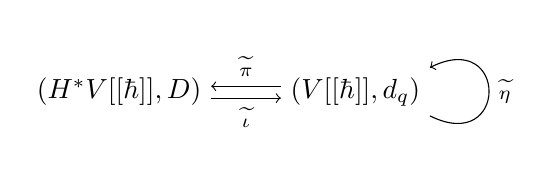
\begin{tikzpicture}[baseline=(L.base),anchor=base,->,auto,swap]
     \path node (L) {$(H^*V [[\hbar]],D)$} ++(3,0) node (M) {$(V[[\hbar]],d_q)$} 
     (M.mid) +(0,.075) coordinate (raise) +(0,-.075) coordinate (lower);
     \draw (L.east |- lower) to node {$\scriptstyle \widetilde{\iota}$} (M.west |- lower);
     \draw (M.west |- raise) to node {$\scriptstyle \widetilde{\pi}$} (L.east |- raise);
     \draw (M.south east) ..controls +(1,-.5) and +(1,.5) .. node {$\scriptstyle \widetilde{\eta}$} (M.north east);
  \end{tikzpicture},
\]
with $D$ something relatively simple. In particular, the projection operator $\widetilde{\pi}$ provides a method for computing the expectation value of an element $f \in V[[\hbar]]$. Namely, $\widetilde{\pi}(f)$ lives in a much smaller complex than $f$, so that its cohomology class is easy to compute explicitly.

Indeed, the main results of section \ref{BV.Wick} can be phrased as ``Feynman diagrams are an implementation of the homological perturbation lemma." We now indicate how to justify that assertion. First, we will outline the proof without writing a formal proof, as it involves combinatorics and algebra that is straightforward but involved. Second, we do an explicit example that demonstrates the requisite computations.

As in section \ref{BV.Wick}, let $V = \RR^N$ and $A = (a_{ij})$ a positive-definite, symmetric, real $N \times N$ matrix. We define
\[
\obscl_I := ( \CC[[x_1, \ldots, x_N, \xi_1, \ldots, \xi_N]], d_I)
\]
where
\[
d_I = -\sum_{i,j = 1}^N a_{ij} x_i\frac{\partial}{\partial \xi_i} + \{I, -\}.
\]
We wish to apply the homological perturbation lemma by adding 
\[
\hbar \Delta_{Leb} = \hbar \sum_{i = 1}^N \frac{\partial}{\partial x_i}\frac{\partial}{\partial \xi_i}
\]
to $d_I$.

As shown in the proof of Wick's lemma (lemma \ref{Wick}), the complex for $I = 0$ is precisely a Koszul complex describing the origin inside $V$ (i.e., arising from the regular sequence given by the rows of $A$). Hence, there is a simple contraction
\[
  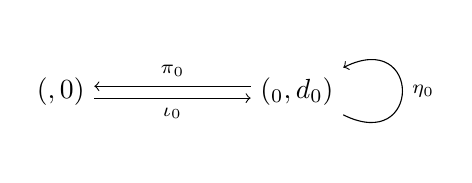
\begin{tikzpicture}[baseline=(L.base),anchor=base,->,auto,swap]
     \path node (L) {$(\CC,0)$} ++(3,0) node (M) {$(\obscl_0,d_0)$} 
     (M.mid) +(0,.075) coordinate (raise) +(0,-.075) coordinate (lower);
     \draw (L.east |- lower) to node {$\scriptstyle \iota_0$} (M.west |- lower);
     \draw (M.west |- raise) to node {$\scriptstyle \pi_0$} (L.east |- raise);
     \draw (M.south east) ..controls +(1,-.5) and +(1,.5) .. node {$\scriptstyle \eta_0$} (M.north east);
  \end{tikzpicture}.
\]
Here $\iota_0$ is the inclusion of $\CC \cong \Sym^0$ into $\obscl$ and $\pi_0$ is projection onto $\Sym^0 \cong \CC$. {\em Note that $\pi_0$ is given by ``evaluation at $0$," where $0$ is the critical point of the quadratic function $\langle x, A x \rangle$.} The homotopy $\eta_0$ can be constructed quite explicitly (see proposition \ref{homotopysym} below).

Wick's lemma is now a direct consequence of the homological perturbation lemma. If we deform the differential on $\obscl[[\hbar]]$ by adding $\hbar \Delta_{Leb}$, we get a new projection map
\begin{align*}
\widetilde{\pi}_0  &= \pi_0 + \pi_0 \circ (\One - \hbar \Delta_{Leb} \eta_0)^{-1} \circ \hbar \Delta_{Leb} \circ \eta_0\\ 
&= \sum_{n \geq 0} \hbar^{n} \pi_0 (\Delta_{Leb} \eta_0)^n.
\end{align*}
Direct calculation verifies that $\widetilde{\pi}_0(x^\nu)$ recovers precisely the formula given in lemma \ref{Wick}.\footnote{As earlier, calculation is quite direct in the case of $V = \RR^1$. For the higher dimensional case, it's easiest to diagonalize $A$ and then take tensor products of the one-dimensional case.} That is, {\em $\widetilde{\pi}_0$ computes the expectation value.} In this homological setting, the fact that $\Delta_{Leb}$ is a constant-coefficient second-order differential operator makes the origins of Wick's lemma a bit clearer: in the perturbation, we lower the polynomial degree by two for every power of $\hbar$. In terms of Feynman diagrams, we are iteratively attaching both ends of a loop.

The differential $\{I,-\}$ is also a small perturbation of $\obscl_0$, so we can construct a homotopy equivalence
\[
  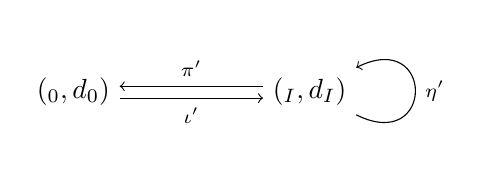
\begin{tikzpicture}[baseline=(L.base),anchor=base,->,auto,swap]
     \path node (L) {$(\obscl_0,d_0)$} ++(3,0) node (M) {$(\obscl_I,d_I)$} 
     (M.mid) +(0,.075) coordinate (raise) +(0,-.075) coordinate (lower);
     \draw (L.east |- lower) to node {$\scriptstyle \iota'$} (M.west |- lower);
     \draw (M.west |- raise) to node {$\scriptstyle \pi'$} (L.east |- raise);
     \draw (M.south east) ..controls +(1,-.5) and +(1,.5) .. node {$\scriptstyle \eta'$} (M.north east);
  \end{tikzpicture},
\]
which composes with the earlier homotopy equivalence $(\pi_0, \iota_0,\eta_0)$ to yield
\[
  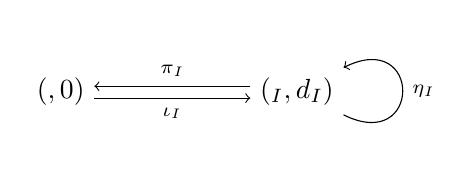
\begin{tikzpicture}[baseline=(L.base),anchor=base,->,auto,swap]
     \path node (L) {$(\CC,0)$} ++(3,0) node (M) {$(\obscl_I,d_I)$} 
     (M.mid) +(0,.075) coordinate (raise) +(0,-.075) coordinate (lower);
     \draw (L.east |- lower) to node {$\scriptstyle \iota_I$} (M.west |- lower);
     \draw (M.west |- raise) to node {$\scriptstyle \pi_I$} (L.east |- raise);
     \draw (M.south east) ..controls +(1,-.5) and +(1,.5) .. node {$\scriptstyle \eta_I$} (M.north east);
  \end{tikzpicture}.
\]
The projection $\pi_I$ is given by iteratively applying an operation that depends on $I$. In terms of Feynman diagrams, this is the tree-level expansion. Again, $\pi_I$ amounts to ``evaluation at the origin, the critical point."

We now perturb by $\hbar \Delta_{Leb}$. Diagrammatically, the new projection is given by iteratively attaching a loop, just as in the case of Wick's lemma. If one draws the diagrams, one sees the Herculean game of Hydra reappear. {\em The projection operator $\widetilde{\pi}_I$ computes the expectation value of any $f \in \obsq_I$.} In other words, the Feynman diagram expansion is just a combinatorial description of this projection operator.

These techniques apply {\it mutatis mutandis} to more general BD algebras, and thus we will obtain a point of view on how Feynman diagrams enter into the study of general QFT. In the next subsection, we discuss the essential algebra before introducing the analytic issues that appear in QFT proper.

\begin{example}
Let $N = 1$. We start with the contraction of classical observables
\[
  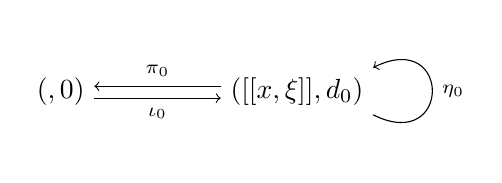
\begin{tikzpicture}[baseline=(L.base),anchor=base,->,auto,swap]
     \path node (L) {$(\CC,0)$} ++(3,0) node (M) {$(\CC[[x,\xi]],d_0)$} 
     (M.mid) +(0,.075) coordinate (raise) +(0,-.075) coordinate (lower);
     \draw (L.east |- lower) to node {$\scriptstyle \iota_0$} (M.west |- lower);
     \draw (M.west |- raise) to node {$\scriptstyle \pi_0$} (L.east |- raise);
     \draw (M.south east) ..controls +(1,-.5) and +(1,.5) .. node {$\scriptstyle \eta_0$} (M.north east);
  \end{tikzpicture}.
\]
Here $\xi$ has degree $-1$ and $d_0 = - ax \partial_\xi$. The homotopy is
\[
\eta_0 (x^n) = 
\left\{ 
\begin{array}{cc}
0, & n = 0\\
\frac{1}{a} x^{n-1}, & n > 0
\end{array}
\right.
\]
as one can quickly check.

Consider the perturbation by $\hbar \Delta_{Leb}$. We compute that
\[
\hbar \Delta_{Leb} \eta_0 (x^n) = 
\left\{ 
\begin{array}{cc}
0, & n = 0,1\\
\frac{\hbar}{a} (n-1) x^{n-2}, & n > 1
\end{array}
\right.
\]
and hence
\[
(\hbar \Delta_{Leb} \eta_0)^m (x^n) = 
\left\{ 
\begin{array}{cc}
0, & n < 2m \\
\left(\frac{\hbar}{a}\right)^m (n-1)(n-3) \cdots (n - (2m-1)) x^{n-2m}, & n \geq 2m
\end{array}
\right. .
\]
We see that
\[
\widetilde{\pi}_0(x^n) = \sum_{m \geq 0} \hbar^n \pi_0(\Delta_{Leb} \eta_0)^m(x^n) = \left\{ 
\begin{array}{cc}
0, & n = 2k \\
\left(\frac{\hbar}{a}\right)^k (2k-1)!!, & n = 2k
\end{array}
\right. .
\]
This is precisely Wick's lemma.

\end{example}

\subsection{The ``free field" case}\label{FFcase}

Much of the rest of this thesis will focus on a situation roughly of the following form, which is a caricature of the ``free field theories" we will study. Let $(V,d)$ be a bounded cochain complex of vector spaces (the ``fields") and set
\[
\sO(T^*[-1]V) := (\Sym(V^\vee \oplus V[1]),d_V),
\] 
the commutative dg algebra where $d$ denotes the obvious differentials on $V^\vee$ and $V[1]$ extended to a derivation. This algebra is ``functions on the shifted cotangent bundle of $V$." The evaluation pairing between $V^\vee$ and $V$ induces a canonical $1$-symplectic pairing that we then extend to a Poisson bracket $\{-,-\}$ by the Leibniz rule. This bracket makes $\sO(T^*[-1]V)$ into a $\P0$ algebra. There is then a canonical BV Laplacian we use to quantize. (We are using the construction from section \ref{BV.Algebra}.)

Now suppose we had a contraction of the linear observables $V^\vee \oplus V[1]$ onto their cohomology $\cH$. We want to obtain a contraction of $\sO(T^*[-1]V)$ onto $\sO(\cH)$ and then use the homotopy perturbation lemma to contract $\obsq$ onto $\sO(\cH)[[\hbar]]$. Thus, our first order of business is to construct a contraction on the symmetric algebras coming from a contraction.

\begin{prop}\label{homotopysym}
Given a contraction
\[
  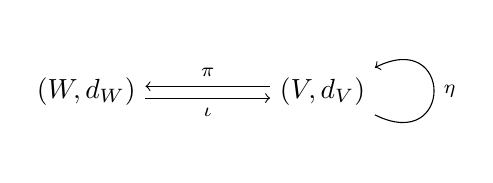
\begin{tikzpicture}[baseline=(L.base),anchor=base,->,auto,swap]
     \path node (L) {$(W,d_W)$} ++(3,0) node (M) {$(V,d_V)$} 
     (M.mid) +(0,.075) coordinate (raise) +(0,-.075) coordinate (lower);
     \draw (L.east |- lower) to node {$\scriptstyle \iota$} (M.west |- lower);
     \draw (M.west |- raise) to node {$\scriptstyle \pi$} (L.east |- raise);
     \draw (M.south east) ..controls +(1,-.5) and +(1,.5) .. node {$\scriptstyle \eta$} (M.north east);
  \end{tikzpicture},
\]
there is a natural contraction on the associated symmetric algebras
\[
  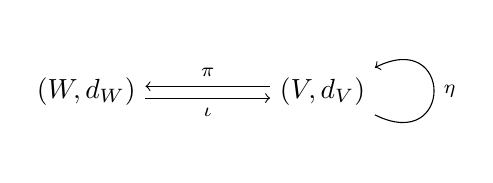
\begin{tikzpicture}[baseline=(L.base),anchor=base,->,auto,swap]
     \path node (L) {$(\Sym W,d_W)$} ++(3,0) node (M) {$(\Sym V,d_V)$} 
     (M.mid) +(0,.075) coordinate (raise) +(0,-.075) coordinate (lower);
     \draw (L.east |- lower) to node {$\scriptstyle \Sym \iota$} (M.west |- lower);
     \draw (M.west |- raise) to node {$\scriptstyle \Sym \pi$} (L.east |- raise);
     \draw (M.south east) ..controls +(1,-.5) and +(1,.5) .. node {$\scriptstyle \Sym \eta$} (M.north east);
  \end{tikzpicture}
\]
where $\Sym \eta$ is constructed explicitly in the proof below.
\end{prop}

\begin{proof}
We elaborate on some simple properties of a contraction that clarify the idea of the proof. First, observe that $\iota \circ \pi$ is a projection operator on the graded module $V$, so we will view $W$ as a submodule of $V$ and denote the projection $P: V \to W \subset V$. The operator $P^\perp = \One_V - P$ is thus also a projection operator, and we denote its image by $W^\perp \subset V$. By construction, $W$ and $W^\perp$ are subcomplexes, i.e., $d_V$ respects the decomposition $V = W \oplus W^\perp$. Second, observe that the side conditions on $\eta$ imply that $\eta$ also respects the decomposition:
\[
P \circ \eta \circ P^\perp = 0 = P^\perp \circ \eta \circ P.
\]
Finally, note that this decomposition implies that $\Sym V \cong \Sym W \ot \Sym W^\perp$. Moreover, $P^\perp$,  extended to a derivation on $\Sym V$, decomposes it into a direct sum of eigen-complexes
\[
\Sym V = \bigoplus_{n \geq 0} M_n \text{ where } M_n = (\Sym W) \ot \Sym^n W^\perp
\]
and $P^\perp$ has eigenvalue $n$ on $M_n$. The map $\One_{\Sym V} - \Sym \iota \circ \Sym \pi$ is then simply the projection of $\Sym V$ onto $\oplus_{n \geq 1} M_n$.

Let $\eta$ denote the operator on $\Sym V$ obtained by extending $\eta$ on $V$ as a derivation. The side conditions imply that $\eta$ respects the eigendecomposition. We now define a map $\Sym \eta$: 
\[
\Sym \eta \big|_{M_n} := \left\{
\begin{array}{ll} 
\frac{1}{n} \eta, & \text{for $n > 0$} \\ 
0, & n = 0
\end{array}
\right. .
\]
It remains to verify $\Sym \eta$ is the desired homotopy.

Observe that the maps $d$, $\eta$, $P^\perp$ all preserve the subcomplexes $\Sym^m W \ot \Sym^n W^\perp$. It is straightforward to verify that, for $n> 0$,
\[
[d, \eta ] \Big|_{\Sym^m W \ot \Sym^n W^\perp} = P^\perp\Big|_{\Sym^m W \ot \Sym^n W^\perp} = n \One_{\Sym^m W \ot \Sym^n W^\perp}
\]
and hence that
\[ 
[d, \Sym \eta ] \Big|_{\Sym^m W \ot \Sym^n W^\perp} = \One_{\Sym^m W \ot \Sym^n W^\perp}.
\]
Thus we see $\Sym \eta$ is the required homotopy.
\end{proof}

Using the same notation as above, suppose we have a complex $(V,d)$ and a contraction for the linear elements of $\sO(T^*[-1]V)$ onto their cohomology $\cH$:
\[
  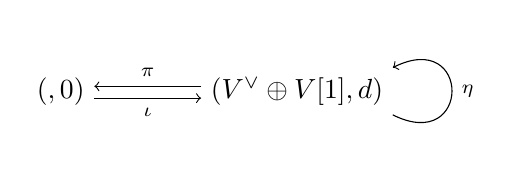
\begin{tikzpicture}[baseline=(L.base),anchor=base,->,auto,swap]
     \path node (L) {$(\cH,0)$} ++(3,0) node (M) {$(V^\vee \oplus V[1],d)$} 
     (M.mid) +(0,.075) coordinate (raise) +(0,-.075) coordinate (lower);
     \draw (L.east |- lower) to node {$\scriptstyle \iota$} (M.west |- lower);
     \draw (M.west |- raise) to node {$\scriptstyle \pi$} (L.east |- raise);
     \draw (M.south east) ..controls +(1,-.5) and +(1,.5) .. node {$\scriptstyle \eta$} (M.north east);
  \end{tikzpicture}.
\]
Let $\Delta$ denote the BV Laplacian on $\Sym(V^\vee \oplus V[1])$. There are two, closely-related perturbations of the classical observables that interest us:
\begin{enumerate}
\item[(a)] the parameter $\hbar$ is not formal (i.e., can take nonzero values)
\[
\obsq := ( \Sym(V^\vee \oplus V[1])[\hbar], d + \hbar \Delta),
\]
\item[(b)] the parameter $\hbar$ is formal (i.e., can take ``infinitesimal" nonzero values)
\[
\obsq := ( \Sym(V^\vee \oplus V[1])[[\hbar]], d + \hbar \Delta).
\]
\end{enumerate}
In either case, $\hbar \Delta$ is a small perturbation. For $\hbar$ formal,  it is clear that the geometric series
\[
(\One - \hbar \Delta \Sym \eta)^{-1} = 1 + \hbar \Delta \Sym \eta + \hbar^2 (\Delta \Sym \eta)^2 + \cdots = \sum_{n \geq 0} \hbar^n (\Delta \Sym \eta)^n
\]
is well-defined. When $\hbar$ is not formal (case (a) above), the same geometric series is well-defined because $\Delta$ is locally nilpotent: if $f \in \Sym^{\leq k}(V^\vee \oplus V[1])$, then $\Delta^m f = 0$ for $2m > k$. 

By the perturbation lemma, we then obtain a perturbation of $\Sym \cH[[\hbar]]$ whose differential is now
\begin{eqnarray*}
D &=& \Sym \pi \circ (\One - \hbar \Delta \Sym \eta)^{-1} \circ (\hbar \Delta) \circ \Sym \iota \\ 
    &=& \hbar \sum_{n \geq 0} \hbar^n \Sym \pi \circ\underbrace{\Delta \Sym \eta \circ \cdots \Delta \Sym \eta}_{\text{with $n$ $\Delta\Sym \eta$'s}} \circ \Delta \circ \Sym \iota.
\end{eqnarray*}
The projection map is
\begin{eqnarray*}
\widetilde{\Sym \pi} & = & \Sym \pi + \Sym \pi \circ (\One - \hbar \Delta \Sym \eta)^{-1} \circ \Delta \circ \Sym \eta \\
 & = &   \sum_{n \geq 0} \hbar^n \Sym \pi \circ \underbrace{\Delta  \Sym \eta \circ \cdots \Delta \Sym \eta}_{\text{with $n$ $\Delta \Sym \eta$'s}} \\
 & = & \Sym \pi \circ (\One - \hbar \Delta \Sym \eta)^{-1}.
\end{eqnarray*}
As in the previous section, {\em this projection map $\widetilde{\Sym \pi}$ is useful because it gives an explicit procedure for computing the expectation value of any $f$ in $\obsq$.} More precisely, it characterizes how to find an element in a smaller complex that is hopefully more manageable.
